\subsection{Dynamic Airspace Sectorisation}

\Gls{DAS} is a responsive approach to airspace management that adjusts sector boundaries according to real-time traffic demand and capacity constraints \cite{Zhou_2023}.
By clustering traffic patterns to identify high-density areas, \gls{DAS} aims to support efficient planning and enhance controller operations \cite{Schultz_2018}.
The key objective is to adapt sector configurations dynamically, in a time-dependent manner, to better match actual operational needs.

Early research on optimising airspace structure applied \glspl{EA}, focusing on balancing controller workload through several operationally relevant metrics, such as the total and standard deviation of task load, geometric coherence of sector shapes and number of flight path intersections caused by sector boundaries \cite{Schultz_2018}.
This approach successfully reproduced existing operational sector designs, such as those in the EDDYDUTA area (Figures \ref{airspace-normal} and \ref{airspace-das}), without relying on expert knowledge.
It also demonstrated adaptability to fluctuating daily traffic patterns (Figure \ref{airspace-dynamic}).


\begin{figure}[!ht]
    \centering
    \begin{subfigure}{.45\textwidth}
        \centering
        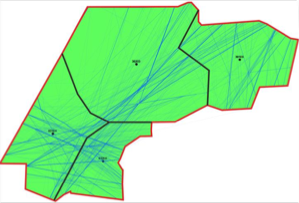
\includegraphics[width=.7\textwidth]{img/airspace.png}
        \caption{Original airspace structure}
        \label{airspace-normal}
    \end{subfigure}
    \begin{subfigure}{.45\textwidth}
        \centering
        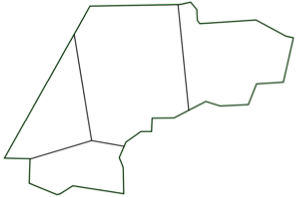
\includegraphics[width=.7\textwidth]{img/airspace-das.png}
        \caption{Sectorisation after \gls{DAS} optimisation}
        \label{airspace-das}
    \end{subfigure}

    \begin{subfigure}{\textwidth}
        \centering
        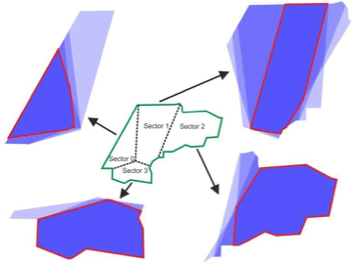
\includegraphics[width=.6\textwidth]{img/airspace-dynamic.png}
        \caption{Dynamic adaptation to traffic demand}
        \label{airspace-dynamic}
    \end{subfigure}

    \caption{Airspace EDDYDUTA \cite{Schultz_2018}}
    \label{airspace}
\end{figure}

Recent research explores deep learning to enhance \gls{DAS}, offering greater scalability and predictive accuracy than traditional \glspl{EA}.
Zhou et al. \cite{Zhou_2022} introduced a \gls{MTL} model using \gls{Bi-LSTM} networks to predict both traffic flow and airspace capacity. 
This model supports proactive sector adjustments based on traffic-capacity imbalance forecasts across multiple time horizons.
While effective, the \gls{Bi-LSTM} model is a black-box system, which limits its operational acceptability due to the lack of transparency in how predictions are derived.

To address this, Zhou et al. \cite{Zhou_2023} proposed a more interpretable \gls{AI} framework called AirFusion, which integrates the \gls{TFT} for time-series forecasting.
The model predicts airspace demand and capacity up to four hours in advance while respecting operational constraints imposed on air traffic controllers.
It incorporates \gls{DBSCAN} clustering to identify major traffic flows and constructs weighted graphs to inform sectorisation decisions.
Results show high predictive accuracy, with mean errors of 0.0234 (demand) and 0.0291 (capacity), and R-squared values of 0.9133 and 0.9605, respectively.
Clustering results are shown in Figure \ref{airspace-tft}, where flight trajectories are color-coded, and major flows within each cluster are indicated by thickened lines. 
When demand exceeds sector capacity, sectors are subdivided (purple dashed lines) to maintain manageable workloads.

\begin{figure}[!ht]
    \centering
    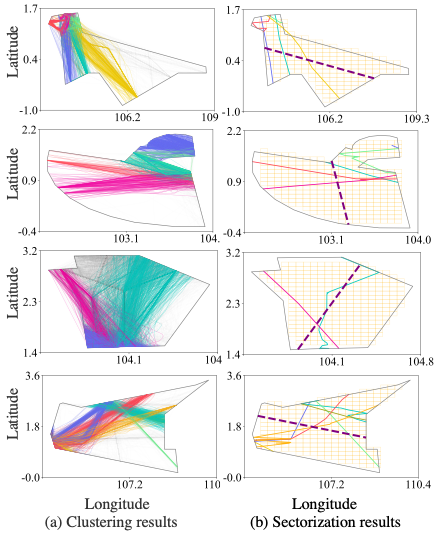
\includegraphics[width=.5\textwidth]{img/airspace-tft.png}
    \caption{Clustering and sectorisation results for selected sectors \cite{Zhou_2023}.}
    \label{airspace-tft}
\end{figure}

Compared to the earlier \gls{Bi-LSTM} approach, the \gls{TFT}-based model offers better interpretability, thanks to integrated feature selection and attention mechanisms. 
This makes it more suitable for operational deployment, where trust and explainability are critical for controller acceptance.


% \Gls{DAS} is a responsive technique used to adjust airspace sector boundaries based on varying traffic demand and airspace capacity \cite{Zhou_2023}. 
% The traffic patterns are clustered to identify areas of high-dense traffic and provide an efficient planning and control structure to support \glspl{ATCO} and users \cite{Schultz_2018}. 
% The goal is to enable airspace sector adaptation in a time-dependent way by dynamically adapting the position and shape of the sectors with respect to actual necessities and restrictions \cite{Schultz_2018}. 

% In the initial research to optimise the airspace structure, \glspl{EA} were applied to optimise the initial airspace structure considering different evaluation functions. 
% In the paper by Schultz \cite{Schultz_2018}, several evaluation functions with different operationally relavent factors have been conprehensively tested:
% \begin{itemize}
%     \item Sum of task load in the investigation scenerio
%     \item Standard deviation of task load
%     \item Well-formed controlling areas, measured by the standard deviation of interior angles
%     \item Number of flight intervals caused by the airspace sectors (intersection of flights).
% \end{itemize}
% With the research work done then, it was shown that it is possible to reproduce the structure of  of operational systems without considering the explicit knowledge of \gls{ATM} experts but aiming at a balanced task load between airspace sectors.
% The original airspace area EDDYDUTA (Figure \ref{airspace-normal}) is optimised with sectorisation similar to the original airspace structure (Figure \ref{airspace-das}).
% Under consideration of the changing traffic demand over the day of operations, the airspace structure will be adopted accordingly (Figure \ref{airspace-dynamic}). 
% Figure \ref{airspace-tft} shows the clustering and sectorisation results for the selected sectors. 
% Each trajectory is colour-coded based on its assigned cluster, with outliers plotted as grey lines. 
% The major flows for each clusters are identified and plotted with thicker lines in Figure \ref{airspace-tft} (b), with boundaries determined by \gls{DAS} indicated by purple dashed lines. 
% These boundaries split each sector into two sub-subsectors, when the demand surpasses the sector's capacity.


% Building onto this idea, \gls{DL} networks are then researched on to improve on \gls{DAS}, as it outperforms \glspl{EA} in adaptability, scalability, and efficiency. 
% Zhou et al \cite{Zhou_2022} proposed a \gls{MTL} approach to predict sector traffic flow and airspace capacity simultaneously using a shared neural network architecture. 
% This study implements \gls{MTL} on \gls{Bi-LSTM} for each prediction tasks, to predict traffic demand-capacity imbalance with respect to different look-ahead time windows and suggests when the two neighbouring airspace sectors can be merged or split.
% Experimental results explicitely show the capacity of the proposed \gls{MTL} model in predicting flow and capacity.
% However, this deep learning method is a ``black box'' model that provide no insight into their input incorporation in practical scenerios, making it for \glspl{ATCO} to trust the prediction results in real-world operations \cite{Zhou_2023}.

% In the subsequent research by Zhou et al \cite{Zhou_2023}, a new machine learning framework AirFusion was design to balance the airspace demand and capacity through \gls{DAS}. 
% This framework differs from the previous with the use of \gls{TFT} to predict air traffic demand and airspace sector capacity with 4-hour look-ahead window, while also taking the account of operational constraints of \glspl{ATCO}.
% It also uses \gls{DBSCAN} techniques to indentify major traffic flows within the selected airspace, thereby formulating selected sectors within this airspace as weighted graphs based on these major flow frequencies. 
% The experimental results demonstrated the model's high accuracy, with a mean error of 0.0234 for traffic demand prediction and 0.0291 for airspace sector capacity prediction.
% Furthermore, the R-squared values indicate high predictive performance, with an average of 0.9133 for traffic demand and 0.9605 for airspace sector capacity.



% The \gls{TFT} model in \cite{Zhou_2023} is a lot more complex compared to \gls{Bi-LSTM} \gls{MTL} model in \cite{Zhou_2022}.
% The \gls{TFT} model is built for interpretable time-series forecasting while the \gls{Bi-LSTM} \gls{MTL} is more generic and lacks integrated feature selection and interpretability. 
